\documentclass[%
    a4paper,                % Tamaño de papel A4.
    twoside,                % Páginas pares e impares con diseño diferenciado.
    12pt,                   % Tamaño de fonte. Non inferior a 12 puntos. 
]{report}                     % Cambiado a "book" para soportar \frontmatter, \mainmatter y \backmatter

\usepackage[english]{babel}
\usepackage{enumitem}
\usepackage{tfmteleco}      % Tu paquete personalizado de la escuela
\usepackage{booktabs}       % Necesario para las tablas profesionales que generamos

\title{ANALYSIS OF CONVERSATIONAL DATA FROM
HEALTH-FOCUSED CHATBOTS USING NATURAL
LANGUAGE PROCESSING TECHNIQUES}
\author{Adrián Bernardo Barrero}
\titores{Francisco Javier González Castaño, Anxo Gesto Gayoso}
\curso{2025/2026}

\setcounter{tocdepth}{2}

\begin{document}

% --- FRONTMATTER: Numeración romana (i, ii, iii...) ---
\frontmatter

\maketitle
\clearemptydoublepage

% Blank page after title page

\newpage
\thispagestyle{empty}
\mbox{}
\addtocounter{page}{-1}

% **************************************************
% * Dedication page
% **************************************************

\newpage
\thispagestyle{empty}

\begin{flushright}
  \emph{To my parents} \\
  \emph{To my whole family} \\
\end{flushright}

\clearemptydoublepage

% **************************************************
% * Acknowledgements page
% **************************************************

\thispagestyle{empty}

\section*{Acknowledgements}

This thesis marks the end of an incredible experience: deciding to come to Vigo to pursue this master’s degree.
What began as a vague idea of what I wanted to do ended up being the consequence of making a decision without the freedom to fully choose it, in rushed circumstances, yet one I do not regret.

I want to begin by thanking my entire family for making it possible, and for their constant support and love.
To GTI, for showing me another side of the University, one that I enjoyed far more than I ever expected.
To all my friends, including those I have met here, but especially to Andrés.


Finally, also to the things that still hurt to have left behind in order to keep moving forward.
Those are the things that taught me what is truly valuable, and helped me find myself.

\begin{flushright}
  \textit{Vigo, \today}
\end{flushright}

\clearemptydoublepage

\clearemptydoublepage

% El Abstract se incluye aquí, antes del índice
\begin{abstract}
This Master’s Thesis investigates the automated detection of self-disclosure in 16,000 chatbot interactions with elderly users. Grounded in Social Penetration Theory, the study evaluates various feature extraction pipelines using the Gemma-2-9b-it LLM. We compare binary versus rubric-based scoring and direct versus subtopic-based classification aggregated via Hadamard products. An unsupervised K-Means clustering approach is employed to identify thematic patterns, moving beyond heuristic metrics to a theory-driven $N+1$ architecture. Validation is conducted against a Gold Standard of 130 manually annotated sessions by four experts, utilizing Krippendorff’s Alpha, F1-score, and MCC. The results provide a robust methodological foundation for monitoring vulnerability and trust-building in conversational AI for senior citizens.

\vspace{0.5cm}
\noindent \textbf{Keywords:} Natural Language Processing, Self-Disclosure, LLM, Social Penetration Theory, K-Means Clustering, Elderly Care.
\end{abstract}
\newpage
\clearemptydoublepage

\tableofcontents
\clearemptydoublepage

\listoffigures
\clearemptydoublepage

\listoftables
\clearemptydoublepage

% --- MAINMATTER: Numeración arábiga (1, 2, 3...) ---
\mainmatter

\section{Introduction}
    \subsection{Motivation and Context}

The progressive aging of the global population has led to a significant increase in social isolation among senior citizens. To address this, AI-driven conversational agents have emerged as a scalable tool for providing companionship and monitoring. However, the effectiveness of these interactions depends on the user's willingness to reveal personal information—a process known as self-disclosure.
 \vspace{2mm} \newline
In the field of psichology, understanding how and when an elderly user shares sensitive details (health, memories, or emotions) is critical. This project is motivated by the need to transform unstructured dialogue data from over 16,000 sessions into actionable insights. By applying Social Penetration Theory and Large Language Models (LLMs), we aim to establish a robust methodology to measure this trust-building process. From a telecommunications engineering perspective, this work addresses the challenge of extracting high-level semantic features to detect vulnerability and improve the quality of human-machine interaction in sensitive contexts.


    \subsection{Problem Statement: Automated Self-Disclosure Detection}

Despite the proliferation of conversational agents for elderly care, there is a lack of robust, automated methods to quantify the emotional and personal depth of these interactions. While current Natural Language Processing (NLP) techniques can handle intent recognition or sentiment analysis, they often fail to capture the nuances of self-disclosure.
\vspace{2mm} \newline
The core challenge lies in the unstructured nature of dialogue data and the subjective complexity of what constitutes a "sensitive" or "deep" revelation. Existing approaches often rely on rigid keyword matching or general-purpose sentiment scores, which are insufficient for identifying the thematic layers (health, relationships, personal history) defined by social psychology. Furthermore, the use of Large Language Models (LLMs) as evaluators introduces a new problem of methodological reliability: there is no consensus on whether binary classification, multi-level rubrics, or subtopic aggregation yields the most accurate representation of user trust. Therefore, this research addresses the need for a validated, theory-driven pipeline to transform raw conversational data into a structured metric of self-disclosure in the context of elderly-AI interaction.






    
    \subsection{Research Objectives}

The primary objective of this thesis is to design and evaluate a methodological pipeline for the automated detection and classification of self-disclosure in dialogues between elderly users and conversational AI, leveraging Large Language Models (LLMs) and unsupervised learning techniques.

To achieve this overarching goal, the following specific objectives have been established:

\begin{description}
    \item[O1: Feature Extraction and Scoring.] To implement and compare different scoring strategies— specifically binary versus rubric-based (0-5) scales—using a model to extract high-level semantic features from 16,000 conversational sessions.
    \item[O2: Methodological Comparison of Classification.] To evaluate the effectiveness of direct category classification versus a bottom-up approach that utilizes subtopic aggregation through the application of \textit{Hadamard products}.
    \item[O3: Unsupervised Pattern Identification.] To perform clustering (\textit{K-Means}) on the extracted features to identify thematic domains based on Social Penetration Theory, justifying the implementation of an $N+1$ cluster architecture.
    \item[O4: Empirical Validation.] To validate the model's performance against a human-annotated Gold Standard of 120 sessions, measuring inter-rater reliability via \textit{Krippendorff’s Alpha} and assessing classification accuracy through \textit{F1-score} and \textit{Matthews Correlation Coefficient (MCC)}.
\end{description}
        
    \subsection{Thesis Structure}


    This document is structured into seven chapters that guide the reader through the theoretical, technical, and evaluative phases of the research:

\begin{itemize}
    \item \textbf{Chapter 2: Theoretical Framework and State of the Art} explores the psychological foundations of Social Penetration Theory and the technical landscape of Large Language Models (LLMs) and unsupervised learning.
    
    \item \textbf{Chapter 3: Dataset Description and Preprocessing} details the characteristics of the conversational dataset and the protocols followed to ensure data privacy and RGPD compliance.
    
    \item \textbf{Chapter 4: Methodology} constitutes the technical core of the thesis, describing the experimental design for feature extraction, the mathematical application of the \textit{Hadamard product} for subtopic aggregation, and the $K$-Means clustering configuration.
    
    \item \textbf{Chapter 5: Analysis of Results} evaluates the outcome of the clustering process, providing a thematic characterization of the identified self-disclosure domains.
    
    \item \textbf{Chapter 6: Validation and Evaluation} assesses the model's performance by comparing it against an expert-annotated Gold Standard, using metrics such as Krippendorff’s Alpha.
    
    \item \textbf{Chapter 7: Conclusions and Future Work} synthesizes the findings, discusses the limitations of the study, and outlines potential applications in the field of elderly care.
\end{itemize}


\subsection{Social Penetration Theory}


Social Penetration Theory (SPT) provides a foundational framework for understanding how individuals reveal personal information to others, a process termed \textit{self-disclosure}. Often illustrated through the "onion metaphor," the theory suggests that personality is structured in layers, and relational development involves the systematic "peeling" of these layers through communication.

According to the theory, the disclosure process is defined by two primary dimensions:
\begin{enumerate}
    \item \textbf{Breadth:} The variety of topics covered during an interaction.
    \item \textbf{Depth:} The level of intimacy or sensitivity of the information shared within those topics.
\end{enumerate}

In the digital era, SPT has been widely adapted to study Human-Computer Interaction (HCI). In this thesis, the theory is utilized to categorize conversational data into distinct thematic domains. By mapping user utterances to specific layers—ranging from superficial biographical data to more intimate disclosures regarding \textit{Health}, \textit{Relationships}, and \textit{Personal Development}—we can quantify the level of trust and openness established between the elderly user and the conversational agent. This theoretical grounding justifies the selection of our classification categories and provides the necessary psychological context for the subsequent unsupervised learning phase.


\subsubsection{The Layered Structure of Disclosure}

Taylor and Altman describe the structure of personality as a series of concentric layers, ranging from the most visible to the most private aspects of an individual. The transition through these layers is what defines the "penetration" process:

\begin{itemize}
    \item \textbf{Peripheral Layer:} Contains "public" or observable data. It includes biographical facts (age, origin) and surface-level preferences. In elderly-agent interactions, this corresponds to the initial exchange of greetings and general information.
    \item \textbf{Intermediate Layer:} Encompasses personal opinions, social attitudes, and historical narratives. While still relatively safe to share, these topics reflect the individual's values and professional or social trajectory.
    \item \textbf{Core Layer:} Represents the most intimate and sensitive domain of the self. It includes deep-seated emotions, vulnerabilities, chronic health concerns, and significant life-changing events (such as widowhood or trauma). 
\end{itemize}

The systematic movement from the peripheral to the core layer is governed by the \textit{norm of reciprocity}, although in Human-Computer Interaction (HCI), this dynamic shifts as the user perceives the agent as a non-judgmental confidant. This study specifically targets the identification of shifts from the intermediate to the core layers, as they are the most indicative of the chatbot's success in fostering a supportive environment for the elderly.



The situational context and the nature of the communication channel significantly influence how self-disclosure is enacted. According to \cite{Bazarova2014}, self-disclosure in digital environments is not merely a direct reflection of relational depth but is also driven by specific functional motivations that vary across different platforms. Their research highlights that the technical affordances of a medium—such as perceived privacy and audience reach—shape the intimacy and characteristics of the shared information. 

In the specific context of this study, this functional approach is crucial: the interaction between an elderly user and a chatbot represents a unique, private communication channel. This perceived intimacy may lower the "social cost" of disclosure, encouraging users to reveal information from the \textit{core layer}—such as chronic health issues or deep personal history—more freely than they would in other digital social settings.


\newpage
\section{Theoretical Framework and State of the Art}

    \subsection{Social Penetration Theory}


Social Penetration Theory (SPT) provides a foundational framework for understanding how individuals reveal personal information to others, a process termed \textit{self-disclosure}. Often illustrated through the "onion metaphor," the theory suggests that personality is structured in layers, and relational development involves the systematic "peeling" of these layers through communication.

According to the theory, the disclosure process is defined by two primary dimensions:
\begin{enumerate}
    \item \textbf{Breadth:} The variety of topics covered during an interaction.
    \item \textbf{Depth:} The level of intimacy or sensitivity of the information shared within those topics.
\end{enumerate}

In the digital era, SPT has been widely adapted to study Human-Computer Interaction (HCI). In this thesis, the theory is utilized to categorize conversational data into distinct thematic domains. By mapping user utterances to specific layers—ranging from superficial biographical data to more intimate disclosures regarding \textit{Health}, \textit{Relationships}, and \textit{Personal Development}—we can quantify the level of trust and openness established between the elderly user and the conversational agent. This theoretical grounding justifies the selection of our classification categories and provides the necessary psychological context for the subsequent unsupervised learning phase.


\subsubsection{The Layered Structure of Disclosure}

Taylor and Altman describe the structure of personality as a series of concentric layers, ranging from the most visible to the most private aspects of an individual. The transition through these layers is what defines the "penetration" process:

\begin{itemize}
    \item \textbf{Peripheral Layer:} Contains "public" or observable data. It includes biographical facts (age, origin) and surface-level preferences. In elderly-agent interactions, this corresponds to the initial exchange of greetings and general information.
    \item \textbf{Intermediate Layer:} Encompasses personal opinions, social attitudes, and historical narratives. While still relatively safe to share, these topics reflect the individual's values and professional or social trajectory.
    \item \textbf{Core Layer:} Represents the most intimate and sensitive domain of the self. It includes deep-seated emotions, vulnerabilities, chronic health concerns, and significant life-changing events (such as widowhood or trauma). 
\end{itemize}

The systematic movement from the peripheral to the core layer is governed by the \textit{norm of reciprocity}, although in Human-Computer Interaction (HCI), this dynamic shifts as the user perceives the agent as a non-judgmental confidant. This study specifically targets the identification of shifts from the intermediate to the core layers, as they are the most indicative of the chatbot's success in fostering a supportive environment for the elderly.



The situational context and the nature of the communication channel significantly influence how self-disclosure is enacted. According to \cite{Bazarova2014}, self-disclosure in digital environments is not merely a direct reflection of relational depth but is also driven by specific functional motivations that vary across different platforms. Their research highlights that the technical affordances of a medium—such as perceived privacy and audience reach—shape the intimacy and characteristics of the shared information. 

In the specific context of this study, this functional approach is crucial: the interaction between an elderly user and a chatbot represents a unique, private communication channel. This perceived intimacy may lower the "social cost" of disclosure, encouraging users to reveal information from the \textit{core layer}—such as chronic health issues or deep personal history—more freely than they would in other digital social settings.
    
    \subsection{Natural Language Processing and Generative AI}

The evolution of Natural Language Processing (NLP) has been marked by a transition from shallow statistical analysis to deep semantic understanding. In the preliminary stages of this study, various traditional NLP libraries were tested, such as \textit{spaCy} for syntactic parsing, \textit{NLTK} and \textit{TextBlob} for basic text processing, and \textit{pysentimiento} for sentiment and emotion detection. 

While these tools provide a solid baseline, they encounter two primary obstacles in the context of this research. First, their performance is notably superior in English-centric datasets, whereas our corpus consists of spontaneous Spanish dialogues, introducing complexities related to syntax, slang, and cultural nuances. Second, traditional models often operate at a surface level, struggling to capture the complex thematic layers defined by Social Penetration Theory.

To overcome these limitations, we transitioned to the use of Large Language Models (LLMs), specifically the \textbf{Gemma-2-9b-it} model. Its architecture is particularly well-suited for this thesis due to its advanced reasoning capabilities and its ability to process Spanish with high semantic fidelity. 
    
        \subsubsection{Evolution of LLMs: The Gemma-2-9b-it Model}

The landscape of Natural Language Processing has been redefined by the advent of Large Language Models (LLMs) that provide high-tier reasoning within accessible hardware requirements. The \textbf{Gemma-2-9b-it} model stands out as a state-of-the-art open-model solution. As detailed by the \cite{https://doi.org/10.48550/arxiv.2408.00118}, the Gemma 2 family introduces architectural optimizations that allow smaller-scale models to outperform significantly larger predecessors in benchmarks involving common sense and reasoning.

In this thesis, the choice of the 9B variant is justified by a dual constraint: hardware limitations and dataset scale. The model was deployed in its native precision (\textit{bfloat16}) to ensure maximum semantic fidelity, as no quantization was applied during loading process from the Hugging Face Hub. The experimental environment is equipped with an \textbf{NVIDIA A10 GPU} (24GB). The memory footprint $M$ for an LLM is a function of its parameter count $P$ and the precision $B$ in bytes:

Given that $P \approx 9.2 \times 10^9$ and $B = 2$ bytes (16 bits), we obtain:

\begin{equation}
    M_{weights} \approx 9.2 \text{ B} \times 2 \text{ bytes} = 18.4 \text{ GB}
\end{equation}
The remaining VRAM is utilized for the \textit{Key-Value (KV) Cache} and activation tensors during \gls{inference}. This leaves a safety margin of approximately 5.6 GB, ensuring stable processing of long conversational contexts without \textit{Out-of-Memory} (OOM) errors.

While this hardware is capable of handling sophisticated inference, the use of larger-scale architectures would result in prohibitive inference times given the volume of our dataset, which comprises \textbf{16,000 sessions}. Thus, Gemma-2-9b-it was selected as it offers the highest "performance-per-parameter" ratio available, ensuring that the processing of the entire Spanish corpus remains computationally feasible without sacrificing semantic depth.

To ensure structural reliability, the \gls{inference} process was constrained by a \textbf{maximum output token limit}. This restriction is possible due to a \textbf{deterministic} output that strictly follows the requested JSON format.

In terms of computational throughput, the processing of the entire dataset exhibited a significant range of latency. Depending on the complexity of the prompt and the specific experiment (A, B, or C), the execution time fluctuated between \textbf{8 hours and 2 days}. These durations reflect the balance between the depth of semantic analysis and the high-volume processing demands of the 2,174 unique user sessions.

Moreover, the model's instruction-tuned (\textit{it}) capabilities are paramount for the feature extraction phase. Research by \cite{10796809} highlights the efficiency of Gemma-based models in following complex prompts and recovering nuanced information from text. This is a critical factor for our study, as the model must interpret the emotional and thematic layers of elderly users' speech in Spanish—a language that often presents dialectal variations and informal structures that traditional, non-generative NLP tools fail to capture accurately.



        
        \subsubsection{LLMs as Feature Extractors in Social Computing}

The field of Social Computing relies on the ability to quantify human behavior through computational lenses. Historically, this has been achieved via programmatic feature extraction, which utilizes deterministic scripts to derive surface-level metrics. In this research, these programmatic features include interaction frequency, average message length, and the identification of proper nouns. While computationally inexpensive and objective, these metrics act only as proxies for social behavior; they fail to capture the underlying meaning or the emotional weight of the discourse.

Large Language Models (LLMs) represent a significant advancement by enabling \textit{Semantic Feature Extraction}. In this paradigm, the model functions as a sophisticated encoder that transforms unstructured text into high-level categorical or numerical scores based on complex rubrics. This study utilizes Gemma-2-9b-it to extract features that were previously inaccessible to traditional NLP, such as:

\begin{itemize}
    \item The sensitivity level of the discussed topics (e.g., political views, health data).
    \item The thematic alignment with the layers of Social Penetration Theory (not used).
    \item The degree of personal revelation within a specific conversational context (not used).
\end{itemize}

The synergy between programmatic and LLM-based features is critical for a comprehensive analysis. Programmatic features provide the structural "skeleton" of the conversation, while LLM-derived features provide the "flesh" or semantic depth. This dual-layered approach allows us to feed the subsequent clustering algorithm with a feature vector that encapsulates both the quantitative dynamics of the interaction and the qualitative nature of the user's self-disclosure.
        
    \subsection{Unsupervised Machine Learning}

Unsupervised machine learning comprises a set of techniques designed to identify underlying structures and patterns in datasets that lack explicit labels. In the context of this thesis, where the objective is to categorize the depth of 16,000 spontaneous interactions without a pre-existing \textit{Gold Standard}, this paradigm provides a scalable and objective framework for behavioral discovery.

Following the comprehensive review by \cite{Naeem2023}, unsupervised learning is fundamental for exploratory data analysis, as it allows for the identification of natural groupings based on feature proximity in a multi-dimensional space. The utility of this approach in social computing lies in its ability to handle high-dimensional semantic vectors—such as those extracted via LLMs—and organize them into interpretable clusters without human bias influencing the initial grouping process.



A critical component of unsupervised learning is the evaluation of the resulting data partitions. Since there is no external label to compare against, \cite{Naeem2023} emphasize the use of internal validation criteria to measure clustering quality:
\begin{itemize}
    \item \textbf{Cohesion:} Measures the degree to which elements within a cluster are similar to one another.
    \item \textbf{Separation:} Evaluates the distinctness between different clusters to ensure they represent unique categories.
    \item \textbf{Validation Metrics:} Indicators such as the \textit{Silhouette Score} (measuring point-to-cluster assignment quality) and the \textit{Davies-Bouldin Index} (evaluating the ratio of within-cluster to between-cluster distances) are utilized to assess the mathematical validity of the model.
\end{itemize}

This theoretical grounding justifies the use of clustering as a primary tool for mapping conversational data to the layers of Social Penetration Theory, providing the necessary metrics to evaluate whether the extracted features are capable of forming stable and meaningful representations of user behavior.
    
        
\subsubsection{K-Means Clustering and Evaluation Metrics}

K-Means is an unsupervised learning technique designed to partition $n$ observations into $K$ clusters, where each observation belongs to the group with the nearest mean (centroid). The mathematical objective is to minimize the \textit{Within-Cluster Sum of Squares} (WCSS):

\begin{equation}
    J = \sum_{j=1}^{K} \sum_{x_i \in C_j} \|x_i - \mu_j\|^2
\end{equation}

To evaluate the validity of the partition and select the optimal number of clusters, this study employs the following metrics and heuristics based on the review by \cite{Naeem2023}:

\begin{itemize}
    \item \textbf{Elbow Method:} Identification of the inflection point in the WCSS curve.
    \item \textbf{Silhouette Score:} A measure of cohesion and separation ranging from -1 to 1.
    \item \textbf{Calinski-Harabasz Index:} The ratio of the sum of between-clusters scatter and within-cluster scatter.
    \item \textbf{Davies-Bouldin Index:} The average maximum similarity index of each cluster with another; lower values signify better separation.
    \item \textbf{Gap Statistics:} A statistical technique that compares cluster dispersion with a uniform reference distribution.
\end{itemize}

% --- Tabla de Métricas para el Estado del Arte ---
\begin{table}[htbp]
\centering
\caption{Summary of Clustering Evaluation Metrics and Optimal Selection Criteria.}
\label{tab:clustering_metrics_simple}
\begin{tabular}{@{}ll@{}}
\toprule
\textbf{Metric / Method} & \textbf{Optimal Value Criterion} \\ \midrule
Elbow Method             & "Knee" or Inflection point       \\
Silhouette Score         & Maximize ($\to 1$)               \\
Calinski-Harabasz Index  & Maximize                         \\
Davies-Bouldin Index     & Minimize                         \\
Gap Statistics           & Maximize                         \\
GMM - BIC                & Minimize                         \\
DBSCAN                   & Density-based (Variable)         \\ \bottomrule
\end{tabular}
\end{table}
% ------------------------------------------------

Furthermore, the study considers \textbf{Gaussian Mixture Models (GMM)} evaluated through the \textbf{Bayesian Information Criterion (BIC)} to balance likelihood and parsimony. Finally, we contrast these with \textbf{DBSCAN}, a density-based approach. While DBSCAN is effective at identifying outliers, it may struggle with the varying densities of semantic layers, reinforcing the choice of a centroid-based approach for the thematic categorization required by Social Penetration Theory.



\subsubsection{Dimensionality Reduction and Visualization}

%The feature vectors extracted from the \textit{Gemma-2-9b-it} model reside in a high-dimensional latent space, which can hinder the performance of centroid-based clustering. To address this, two complementary techniques are integrated into the analytical pipeline: Principal Component Analysis (PCA) and t-Distributed Stochastic Neighbor Embedding (t-SNE).

%\textbf{Principal Component Analysis (PCA)} is applied as a deterministic dimensionality reduction step. By performing an eigendecomposition of the covariance matrix, PCA projects the semantic features into a lower-dimensional space that retains the highest possible variance. This reduction not only decreases the computational burden on the K-Means algorithm but also filters out redundant information, emphasizing the primary dimensions of user self-disclosure.

%hile PCA preserves global variance, \textbf{t-SNE} is employed for its superior ability to represent local relationships in a visualizable 2D space. t-SNE converts similarities between data points into joint probabilities and seeks to minimize the Kullback-Leibler divergence between the original and the low-dimensional distributions. In this research, t-SNE serves as a qualitative validation tool, allowing for the visual inspection of the clusters and ensuring that the mathematical partitions reflect coherent patterns of interaction between the elderly users and the chatbot.


The feature vectors extracted from the \textit{Gemma-2-9b-it} model are processed within their original high-dimensional latent space to ensure the theoretical integrity of the SPT categories. To avoid the loss of granular information, \textbf{K-Means clustering is applied directly to the extracted features} without prior reduction. Consequently, dimensionality reduction techniques are used strictly for \textit{post-hoc} analysis and visualization.

\textbf{Principal Component Analysis (PCA)} is implemented as a deterministic validation tool. By projecting the dataset into its primary eigenvectors, PCA allows for the inspection of the global data structure and the verification of cluster separability based on maximum variance.

Furthermore, \textbf{t-Distributed Stochastic Neighbor Embedding (t-SNE)} is utilized to represent complex, non-linear local relationships in a 2D plane. In this pipeline, \textbf{t-SNE serves exclusively as a qualitative visual aid}. It is crucial to denote that neither PCA nor t-SNE are used to feed the clustering algorithm; their role is to provide a human-interpretable validation of the high-dimensional mathematical partitions, ensuring they reflect coherent interaction patterns.



\begin{table}[htbp]
\centering
\caption{Comparison between PCA and t-SNE for Dimensionality Reduction.}
\label{tab:pca_vs_tsne}
\begin{tabular}{@{}lll@{}}
\toprule
\textbf{Feature}          & \textbf{PCA}                  & \textbf{t-SNE}                 \\ \midrule
\textbf{Type}             & Linear                        & Non-linear                     \\
\textbf{Data Preservation}& Global structure (Variance)   & Local structure (Similarity)   \\
\textbf{Computational Cost}& Low / Efficient               & High / Iterative               \\
\textbf{Determinism}      & Deterministic                 & Stochastic (Non-deterministic) \\
\textbf{Output}           & Principal Components          & Low-dimensional clusters       \\
\textbf{Main Use Case}    & Noise reduction / Processing  & Data visualization             \\ \bottomrule
\end{tabular}
\end{table}

\newpage
        
    \subsection{Ethics and Privacy in Sensitive Data Analysis}

    The analysis of natural language in interactions with elderly users presents significant challenges regarding data privacy and ethical handling. This study implements a "Privacy by Design" approach to ensure compliance with security standards and the protection of sensitive information.

\begin{itemize}
    \item \textbf{Local Infrastructure:} A critical security measure in this research is the use of a localized inference pipeline. By deploying the \textit{Gemma-2-9b-it} model on an internal \textbf{NVIDIA A10} server, the need for third-party Cloud APIs was eliminated. This prevents the transmission of unstructured conversational data to external entities, ensuring that the processing remains within a secure and audited environment.
    
    \item \textbf{Data Anonymization and Traceability:} The dataset is structured around unique session and user identifiers (UUIDs), devoid of any direct personal identifiers such as names or contact information. Although no automated Named Entity Recognition (NER) pre-processing was applied to the raw text, the risk of re-identification is mitigated by the restricted access to the dataset and the fact that metadata is limited to technical variables (e.g., timestamps, platform type, and game modes).
    
    \item \textbf{Commitment and Compliance:} All researchers involved in this project have signed a Non-Disclosure Agreement (NDA) to guarantee the confidentiality of the interactions. The ethical responsibility regarding the General Data Protection Regulation (GDPR) and the management of user consent remains with the providing entity, which authorized the use of this data for research and development purposes.
\end{itemize}

This framework ensures that the pursuit of technical innovation in social computing does not compromise the fundamental rights of a vulnerable demographic.


\subsection{Work Hypotesis}

\label{sec:hypothesis}

The present research is built upon the premise that current nlp frameworks for elderly-chatbot interactions often overlook the psychological depth and the temporal evolution of human relationships. By integrating SPT with state-of-the-art Generative Artificial Intelligence (GAI), this project proposes a shift from purely functional dialogue analysis to a multidimensional evaluation of emotional intimacy.

The central hypotheses guiding this work are as follows:

\begin{itemize}
    \item \textbf{H1: Semantic Depth through SPT.} The application of Social Penetration Theory to conversational datasets involving elderly users will reveal patterns of self-disclosure that standard nlp metrics fail to capture. This represents a pioneer application of spt within an nlp framework specifically tailored for the elderly population.
    
    \item \textbf{H2: Superiority of GAI-ML Hybridization.} A hybrid approach---utilizing LLMs for granular subtopic extraction and traditional Machine Learning for clustering---will provide a more robust and interpretable characterization of user profiles than previous precedents.
    
    \item \textbf{H3: Resilience of the Gating Mechanism.} The implementation of a \textbf{Hadamard Product} between rubric-based intensity and binary detection (\textit{Experiment A}) will significantly reduce semantic noise, providing a high-fidelity representation of the user's latent disclosure space.
\end{itemize}

\section{Methodology: Experimental Design}

\subsection{Data Source and preproccesing: 16,301 Conversations with Elderly Users}

The initial stage of this research involved the curation of a large-scale conversational corpus. The raw data comprised approximately 30,561 sessions; however, to ensure the reliability of the self-disclosure analysis, a multi-stage preprocessing pipeline was applied to refine the dataset.

\begin{enumerate}
    \item \textbf{Filtering of Ludic Interactions:} Messages categorized under the \texttt{intent == games} label (e.g., riddles, word searches) were removed. These interactions are governed by rigid game logic rather than spontaneous social exchange, making them unsuitable for studying natural self-revelation.
    \item \textbf{System Message Cleaning:} Technical artifacts, such as the automated response \texttt{(pensando...)} generated during system latency, were purged. This ensures that the subsequent Natural Language Processing (NLP) tasks are performed strictly on human and intentional bot-generated content.
    \item \textbf{Minimal Interaction Constraint:} A threshold was set to exclude sessions with fewer than five total exchanges (human-bot turns). This criterion ensures that only sessions with enough conversational "mass" to exhibit depth are included in the study.
\end{enumerate}



As a result of this process, the final dataset was reduced to \textbf{16,301 valid sessions}. For data management purposes, each session was mapped from a composite identifier \newline \texttt{'\{user\_id\}\_\{session\_id\}.csv'}. This structured approach allows for efficient feature engineering while maintaining the integrity of the original conversational flows.


Beyond the total number of sessions, the dataset comprises \textbf{2,174 unique users}. The relationship between users and their respective number of interactions provides insight into the engagement patterns of the elderly population with the AI system.

\begin{figure}[htbp]
    \centering
    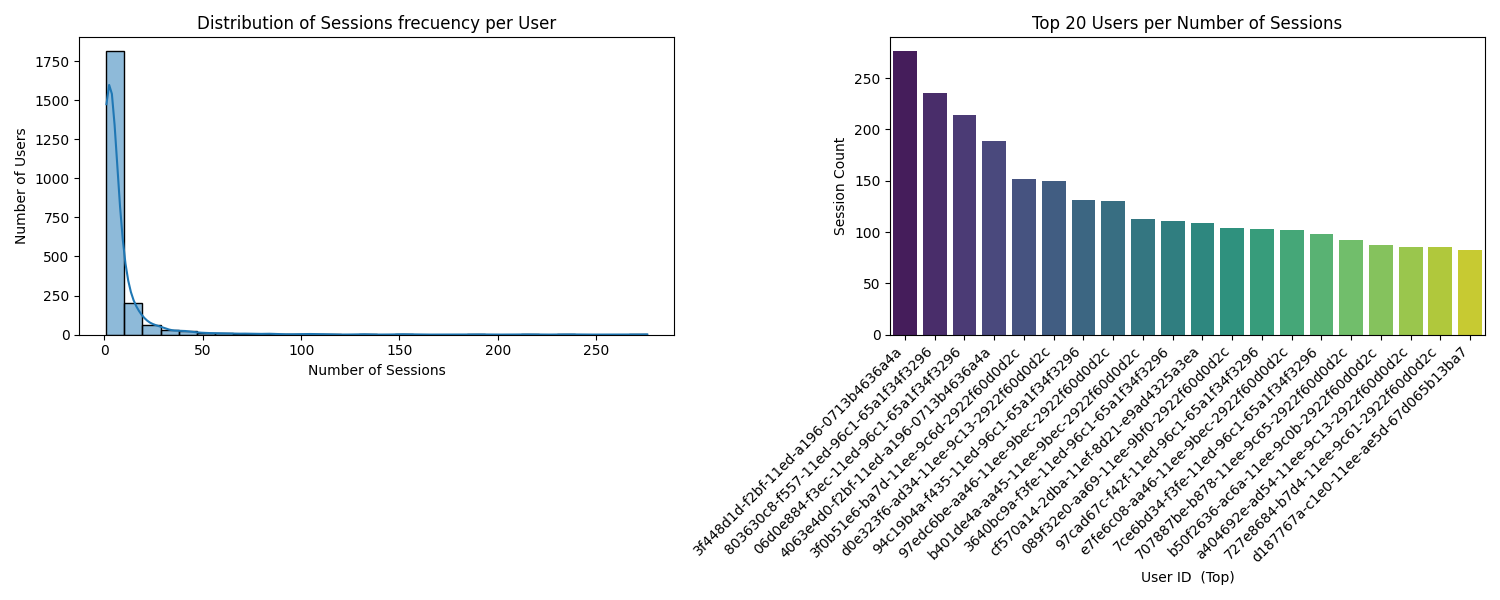
\includegraphics[width=0.8\textwidth]{images/user_dist.png}
    \caption{Distribution of the number of conversations per user (Top 20 most active users).}
    \label{fig:user_dist}
\end{figure}

As shown in Figure \ref{fig:user_dist}, there is a significant variance in user activity. This concentration of data in the most active users allows for a robust analysis of conversational depth, as these long-term interactions are more likely to transition from superficial "cliché" exchanges to more intimate layers of disclosure.

    \newpage
    \subsection{Programmatic Feature Engineering}

In addition to the semantic evaluation, a quantitative characterization of the sessions was performed through programmatic feature engineering. This process involved the extraction of objective metrics that describe the structural, temporal, and emotional dynamics of the human-computer interaction. While the semantic layers focus on \textit{what} is being said, these features provide crucial context on \textit{how} the interaction unfolds.

The engineered features can be categorized into three main groups:
\begin{itemize}
    \item \textbf{Structural and Temporal:} Metrics such as \texttt{session\_duration} and \texttt{n\_user\_interactions} quantify the level of engagement and the length of the conversational exchange.
    \item \textbf{Linguistic Complexity:} Features like \texttt{len\_user\_interactions} and \texttt{n\_proper\_nouns} serve as proxies for the richness of the discourse, where a higher density of proper nouns often correlates with the mention of specific personal entities or anecdotes.
    \item \textbf{Affective Analysis:} Sentiment scores (\texttt{pos}, \texttt{neu}, \texttt{neg}) were calculated for both the user and the bot. Comparing these allows for the assessment of emotional reciprocity, a key component in deepening social penetration.
\end{itemize}

\begin{table}[htbp]
\centering
\caption{Description of Programmatically Engineered Features.}
\label{tab:programmatic_features}
\begin{tabular}{@{}ll@{}}
\toprule
\textbf{Feature Name} & \textbf{Description}  \\ \midrule
\texttt{session\_duration} & Total duration of the session in seconds or minutes. \\
\texttt{n\_user\_interactions} & Total number of interactions initiated by the user. \\
\texttt{percentage\_user\_interactions} & User's share of interactions relative to the session total.  \\
\texttt{len\_user\_interactions} & Average length of the user's messages/inputs. \\
\texttt{n\_proper\_nouns} & Number of proper nouns detected in the conversation.\\
\texttt{user\_sent\_pos} & Positive sentiment score in the user's messages.\\
\texttt{user\_sent\_neu} & Neutral sentiment score in the user's messages. \\
\texttt{user\_sent\_neg} & Negative sentiment score in the user's messages. \\
\texttt{bot\_sent\_pos} & Positive sentiment score in the bot's responses. \\
\texttt{bot\_sent\_neu} & Neutral sentiment score in the bot's responses. \\
\texttt{bot\_sent\_neg} & Negative sentiment score in the bot's responses. \\ \bottomrule
\end{tabular}
\end{table}
    \subsection{Operationalizing Self-Disclosure Categories}

We have defined three primary categories that aggregate various conversational themes. These categories serve as proxies for the breadth and depth of the users' "social personality" layers:

\begin{itemize}
    \item \textbf{Category 1: Health and Well-being.} Focuses on the most immediate and vital concerns of the elderly population. It includes \textit{Mental and Emotional Health} as well as \textit{Physical Health and Addictions}.
    \item \textbf{Category 2: Interpersonal Relationships.} Maps the user's social circle and support system, encompassing \textit{Family Dynamics} and \textit{Affective/Romantic Relationships}.
    \item \textbf{Category 3: History and Personal Development.} Represents the deepest layers of the "onion," covering \textit{Personal Goals and Failures}, \textit{Traumas and Adversity}, and \textit{Professional Life and Career}.
\end{itemize}

\begin{table}[htbp]
\centering
\caption{Operationalized SPT Categories and Sub-themes.}
\label{tab:spt_categories}
\begin{tabular}{@{}ll@{}}
\toprule
\textbf{Main Category} & \textbf{Sub-themes / Dimensions} \\ \midrule
\textbf{C1: Health \& Well-being} & Mental Health, Emotional State, Physical Health, Addictions \\
\textbf{C2: Interpersonal Rel.} & Family Dynamics, Affective Relationships \\
\textbf{C3: Personal Development} & Goals \& Failures, Traumas \& Adversity, Career History \\ \bottomrule
\end{tabular}
\end{table}

This categorization allows the model to assign a numerical score to each session based on the presence and intensity of these topics, effectively creating a "disclosure profile" for every interaction.

    
    \subsection{LLM-Based Feature Extraction (Gemma-2-9b-it)}

The semantic characterization of the corpus was approached through three distinct experiments. These setups aim to compare how different levels of abstraction and scoring methods impact the model's ability to cluster users according to the Social Penetration Theory.

\begin{table}[htbp]
\centering
\caption{Summary of LLM-Based Feature Extraction Experiments.}
\label{tab:llm_experiments}
\begin{tabular}{@{}lp{6cm}p{4.5cm}@{}}
\toprule
\textbf{Experiment} & \textbf{Objective} & \textbf{Methodology} \\ \midrule
\textbf{4.2.3: Exp. A} & Integration of intensity and presence via \textbf{Hadamard Product}. & Rubric (0-5) $\odot$ Binary (0/1) at subcategory level. \\
\textbf{4.2.2: Exp. B} & Direct comparison of scoring granularity at the \textbf{Category level}. & Rubric vs. Binary evaluation for C1, C2, and C3. \\
\textbf{4.2.1: Exp. C} & Fine-grained analysis of \textbf{Subtopics}. & Rubric vs. Binary evaluation for individual subtopics. \\ \bottomrule
\end{tabular}
\end{table}



To ensure consistency between the computational implementation and the analytical results, a standardized nomenclature was established for the six experimental variants. These are grouped into three main categories based on their granularity (Category vs. Subtopic) and their scoring logic (Rubric, Binary, or Hadamard Fusion).

\begin{table}[htbp]
\centering
\caption{Technical nomenclature of the experiments conducted.}
\label{tab:experiment_names}
\begin{tabular}{@{}cllp{5cm}@{}}
\toprule
\textbf{Exp.} & \textbf{ID} & \textbf{Technical Name} & \textbf{Description} \\ \midrule
\textbf{A} & 1 & \texttt{rubric based hadamard fusion} & Category-level rubric scores. \\
           & 2 & \texttt{binary hadamard fusion} & Category-level scores from binary flags. \\ \midrule
\textbf{B} & 3 & \texttt{topic rubric} & Direct evaluation of the 3 main categories using a 0-5 scale. \\
           & 4 & \texttt{topic binary} & Direct presence/absence detection of the 3 main categories. \\ \midrule
\textbf{C} & 5 & \texttt{subtopic rubric} & Detailed 0-5 scoring for each specific sub-dimension. \\
           & 6 & \texttt{subtopic binary} & Presence/absence detection for each specific sub-dimension. \\ \bottomrule
\end{tabular}
\end{table}



\textbf{Experiment A} represents our primary approach, where we hypothesize that multiplying the rubric score by a binary flag (Hadamard Product) filters out low-confidence model assignments while preserving the intensity of high-quality disclosures.\\
\textbf{Experiments B and C} serve as ablation studies and validation baselines to justify the complexity of the feature engineering process.


        \subsubsection{Experiment C: Subtopics (Rubric vs Binary)}
The experimental workflow follows a bottom-up structure, beginning with \textbf{Experiment C (Subtopics)} due to a critical data dependency. This experiment serves as the foundational feature extraction layer; it is a mathematical prerequisite to obtain granular scores for each specific sub-dimension before executing higher-level operations.

The evaluation of subtopics was operationalized through a zero-shot/few-shot hybrid prompt. This prompt defines the semantic boundaries for each of the seven subtopics and establishes a rigorous scoring rubric. Below is the technical implementation of the system prompt used:

\begin{lstlisting}[language=json, caption={System Prompt for Subtopic Feature Extraction.}, label={lst:prompt_subtopics}, frame=single, basicstyle=\small\ttfamily, breaklines=true]
<start_of_turn>user
You are a text analysis system. Your goal is to quantify the level of self-disclosure in a predefined list of topics:
- Health (Mental/Physical)
- Relationships (Family/Affective)
- Personal History (Goals, Traumas, Career)

Analyze the [MESSAGES TO EVALUATE] and assign a score (0-5) to EACH topic. 
Response must be ONLY a valid JSON object.

# EVALUATION SCALE (0-5)
* 0: No Mention.
* 1: Impersonal Mention (General talk).
* 2: Vague Personal Mention (General identification).
* 3: Specific Action Disclosure (Concrete habits/actions).
* 4: Detailed Disclosure (Sharing reasoning/beliefs).
* 5: Deep Disclosure (Vulnerability, impact, deep emotions).

# EXPECTED JSON FORMAT
{
  "mental_emotional_health": Int,
  "physical_health_addictions": Int,
  "family_dynamics": Int,
  "affective_relationships": Int,
  "personal_goals_failures": Int,
  "traumas_adversities": Int,
  "professional_career": Int
}

[MESSAGES TO EVALUATE]: 
<end_of_turn>
\end{lstlisting}

For the binary variant of Experiment C, the model's instructions were simplified to a detection task. The prompt explicitly forbids intermediate values, forcing a strictly boolean output (0 or 1). This reduction in dimensionality serves to minimize variance and provide a high-confidence indicator of thematic occurrence.

\begin{lstlisting}[language=json, caption={System Prompt for Binary Subtopic Detection.}, label={lst:prompt_binary}, frame=single, basicstyle=\small\ttfamily, breaklines=true]
<start_of_turn>user
You are a high-precision text classification system. Your task is to detect the PRESENCE or ABSENCE of specific self-disclosure topics in the provided text.

Analyze the [MESSAGES TO EVALUATE] and assign a value of 1 if the topic is mentioned (regardless of its depth) and 0 if it is not mentioned at all.
Your response must be ONLY a valid JSON object.

# TOPICS TO DETECT
- mental_emotional_health
- physical_health_addictions
- family_dynamics
- affective_relationships
- personal_goals_failures
- traumas_adversities
- professional_career

# DETECTION RULES
* 0: There is no trace of the topic in the text.
* 1: The topic is present in the text (even if vaguely mentioned).

# EXPECTED JSON FORMAT
{
  "mental_emotional_health": 0 or 1,
  "physical_health_addictions": 0 or 1,
  "family_dynamics": 0 or 1,
  "affective_relationships": 0 or 1,
  "personal_goals_failures": 0 or 1,
  "traumas_adversities": 0 or 1,
  "professional_career": 0 or 1
}

[MESSAGES TO EVALUATE]:
<end_of_turn>
\end{lstlisting}



        
        \subsubsection{Experiment A: Rubric-Based vs. Binary Scoring via Hadamard Product}

The hadamard product is used to merge the qualitative depth of the scores.

Given two vectors of dimension $n$, $\mathbf{R}$ (representing rubric scores) and $\mathbf{B}$ (representing binary inclusion to category), the Hadamard product $\odot$ is defined as:
\begin{equation}
    \mathbf{F} = \mathbf{R} \odot \mathbf{B}
\end{equation}

Where each component of the resulting fused vector $\mathbf{F}$ is calculated as:
\begin{equation}
    f_{i} = r_{i} \times b_{i} \quad \text{for  } i = 1, \dots, n
\end{equation}

In matrix-vector form, the operation is represented as:
\begin{equation}
    \begin{bmatrix} r_1 \\ r_2 \\ \vdots \\ r_n \end{bmatrix} \odot \begin{bmatrix} b_1 \\ b_2 \\ \vdots \\ b_n \end{bmatrix} = \begin{bmatrix} r_1 \cdot b_1 \\ r_2 \cdot b_2 \\ \vdots \\ r_n \cdot b_n \end{bmatrix}
\end{equation}

This approach implements a \textit{gating mechanism} where the binary vector $\mathbf{B}$ validates the presence of the category. 

\begin{lstlisting}[language=Python, caption={Mapping of Subtopics to SPT Categories.}, label={lst:mapping_categories}, frame=single, basicstyle=\small\ttfamily]
category_mapping = {
    'Category 1: Health and Well-being': [
        'mental_emotional_health', 
        'physical_health_addictions'
    ],
    'Category 2: Interpersonal Relationships': [
        'family_dynamics', 
        'affective_relationships'
    ],
    'Category 3: Personal History and Development': [
        'personal_goals_failures', 
        'traumas_adversities', 
        'professional_career'
    ]
}
\end{lstlisting}


        
        \subsubsection{Experiment B: Direct Category Evaluation (Rubric vs Binary)}

The rubric-based prompt for Experiment B provides the model with a nuanced scale to differentiate between impersonal mentions and deep emotional vulnerability. This allows for a direct comparison with the aggregated results of Experiment A to determine if "direct inference" leads to a loss of granularity.

\begin{lstlisting}[language=json, caption={System Prompt for Direct Category Rubric Evaluation.}, label={lst:prompt_exp_b_rubric}, frame=single, basicstyle=\small\ttfamily, breaklines=true]
<start_of_turn>user
You are a text analysis system. Your goal is to quantify the level of self-disclosure in a predefined list of categories focused on lived experiences and the author's inner world.

Analyze the [MESSAGES TO EVALUATE] and assign a score (0-5) to EACH category.
Response must be ONLY a valid JSON object.

# CATEGORIES TO EVALUATE
* 'Category 1: Health and Well-being': Includes physical, mental, and emotional health.
* 'Category 2: Interpersonal Relationships': Includes family dynamics and affective relationships.
* 'Category 3: Personal History and Development': Includes goals, failures, traumas, and career.

# EVALUATION SCALE (0-5)
* 0: No Mention.
* 1: Impersonal Mention (General discussion, no personal link).
* 2: Vague Personal Mention (General identification or labels).
* 3: Specific Action Disclosure (Concrete habits or specific actions)
* 4: Detailed Disclosure (Reasoning, beliefs, or specific data).
* 5: Deep Disclosure (Vulnerability, fear, or profound personal impact).

# EXPECTED JSON FORMAT
{
    "Category 1: Health and Well-being": Int,
    "Category 2: Interpersonal Relationships": Int,
    "Category 3: Personal History and Development": Int
}

[MESSAGES TO EVALUATE]: 
<end_of_turn>
\end{lstlisting}

        
The prompt for Experiment B (Binary) instructs the model to act as a high-level classifier. Unlike the subtopic prompt, this version requires the LLM to perform an internal aggregation, considering various aspects (e.g., physical health and emotional state) under a single categorical label.

\begin{lstlisting}[language=json, caption={System Prompt for Direct Category Binary Evaluation.}, label={lst:prompt_exp_b}, frame=single, basicstyle=\small\ttfamily, breaklines=true]
<start_of_turn}user
You are a text analysis system. Your goal is to quantify the level of self-disclosure in a predefined list of broad categories:
- Category 1: Health and Well-being (Mental, emotional, and physical health)
- Category 2: Interpersonal Relationships (Family dynamics, affective relationships).
- Category 3: Personal History and Development (Goals, failures, traumas, career).

Analyze the [MESSAGES TO EVALUATE] and assign a 0 or 1 to EACH category.
Response must be ONLY a valid JSON object.

# BINARY EVALUATION SCALE (0-1)
* 0: No Mention or Not Relevant: The topic is not mentioned or not linked personally.
* 1: Specific Action/Deep Disclosure: The author reveals a concrete habit, action, or reflects deeply on the topic.

# EXPECTED JSON FORMAT
{
    "Category 1: Health and Well-being": 0 or 1,
    "Category 2: Interpersonal Relationships": 0 or 1,
    "Category 3: Personal History and Development": 0 or 1
}

[MESSAGES TO EVALUATE]: 
<end_of_turn>
\end{lstlisting}


    \subsection{Clustering Strategy}
        \subsubsection{Implementation of the K-Means Algorithm}
        \subsubsection{Justification of the N+1 Cluster Architecture}
\section{Methodology: Experimental Design}
    \subsection{Operationalizing Self-Disclosure Categories}
    \subsection{LLM-Based Feature Extraction (Gemma-2-9b-it)}
        \subsubsection{Experiment A: Rubric-Based (0-5) vs. Binary Scoring}
        \subsubsection{Experiment B: Direct Category Evaluation vs. Subtopic Aggregation}
    \subsection{Feature Fusion via Hadamard Product}
    \subsection{Clustering Strategy}
        \subsubsection{Implementation of the K-Means Algorithm}
        \subsubsection{Justification of the N+1 Cluster Architecture}
\section{Analysis of Results}
    \subsection{Comparative Analysis of Feature Extraction Experiments}
    \subsection{Cluster Characterization and Centroid Analysis}
    \subsection{Latent Space Visualization and Inter-Cluster Distances}
\section{Validation and Model Evaluation}
    \subsection{Manual Labeling Protocol and Gold Standard Selection}
    \subsection{Inter-Rater Reliability: Krippendorff's Alpha Analysis}
    \subsection{Human-LLM Cross-Validation}
        \subsubsection{Performance Metrics: F1-Score, MCC, and Classification Accuracy}
    \subsection{Discussion: Discrepancy Analysis and LLM Bias}
\section{Conclusions and Future Work}
    \subsection{Summary of Methodological Findings}
    \subsection{Practical Implications for Vulnerability Detection}
    \subsection{Research Limitations}
    \subsection{Lines for Future Investigation}

% --- BACKMATTER: Bibliografía ---
\backmatter

\bibliographystyle{IEEEtran} 
\nocite{*}
\bibliography{bibliography}
\clearemptydoublepage

% --- APÉNDICES ---
\appendix
\include{appendix}

\end{document}